%----------------------------------------------------------------
%
%  File    :  thesis.tex
%
%  Authors :  Keith Andrews, IICM, TU Graz, Austria
%             Manuel Koschuch, FH Campus Wien, Austria
%			  Sebastian Ukleja, FH Campus Wien, Austria
%             Henrik Schulz, FH Campus Wien, Austria
% 
%  Created :  22 Feb 96
% 
%  Changed :  11 Mar 2024
%
%  For suggestions and remarks write to: sebastian.ukleja@fh-campuswien.ac.at
% 
%----------------------------------------------------------------

% --- Setup for the document ------------------------------------

%Class for a book like style:
\documentclass[11pt,a4paper,oneside]{scrbook}
%For a more paper like style use this class instead:
%\documentclass[11pt,a4paper,oneside]{thesis}

%input encoding for windows in utf-8 needed for Ä,Ö,Ü etc..:
\usepackage[utf8]{inputenc}
%input encoding for linux:
%\usepackage[latin1]{inputenc}
%input encoding for mac:
%\usepackage[applemac]{inputenc}

\usepackage[english]{babel}
% for german use this line instead:
%\usepackage[ngerman]{babel}

%needed for font encoding
\usepackage[T1]{fontenc}
\usepackage{setspace}

% want Arial? uncomment next two lines...
%\usepackage{uarial}
%\renewcommand{\familydefault}{\sfdefault}

%some formatting packages
\usepackage[bf,sf]{subfigure}
\renewcommand{\subfigtopskip}{0mm}
\renewcommand{\subfigcapmargin}{0mm}

%For better font resolution in pdf files
\usepackage{lmodern}

\usepackage{url}

%\usepackage{latexsym}

\usepackage{geometry} % define pagesize in more detail


\usepackage{colortbl} % define colored backgrounds for tables

\usepackage{courier} %for listings
\usepackage{listings} % nicer code formatting
\lstset{basicstyle=\ttfamily,breaklines=true}

\usepackage{graphicx}
  \pdfcompresslevel=9
  \pdfpageheight=297mm
  \pdfpagewidth=210mm
  \usepackage[         % hyperref should be last package loaded
    pdftex, 		   % needed for pdf compiling, DO NOT compile with LaTeX
    bookmarks,
    bookmarksnumbered,
    linktocpage,
    pagebackref,
    pdfview={Fit},
    pdfstartview={Fit},
    pdfpagemode=UseOutlines,                 % open bookmarks in Acrobat
  ]{hyperref}
\DeclareGraphicsExtensions{.pdf,.jpg,.png}
\usepackage{bookmark}

\usepackage[title]{appendix}

%paper format
\geometry{a4paper,left=30mm,right=25mm, top=30mm, bottom=30mm}

% --- Settings for header and footer ---------------------------------
\usepackage{scrlayer-scrpage}
\clearscrheadfoot
\pagestyle{scrheadings}
\automark{chapter}

%Left header shows chapter and chapter name, will not display on first chapter page use \ihead*{\leftmark} to show on every page
\ihead{\leftmark} 	
%\ohead*{\rightmark}	%optional right header
\ifoot*{Student}		%left footer shows student name
\ofoot*{\thepage}		%right footer shows pagination
%---------------------------------------------------------------------

%Start of your document beginning with title page
\begin{document}


% --- Main Title Page ------------------------------------------------
\begin{titlepage}
\frontmatter

\begin{picture}(50,50)
\put(-70,40){\hbox{
\includegraphics{images/logo.png}}}
\end{picture}

\vspace*{-5.8cm}

\begin{center}

\vspace{6.2cm}

\hspace*{-1.0cm} {\LARGE \textbf{Constructing a Zero-Trust Kubernetes Cluster\\}}
\vspace{0.2cm}

\vspace{2.0cm}

\hspace*{-1.0cm} { \textbf{Bachelor Thesis\\}}

\vspace{0.65cm}

\hspace*{-1.0cm} Submitted in partial fulfillment of the requirements for the degree of \\

\vspace{0.65cm}

\hspace*{-1.0cm} \textbf{Bachelor of Science in Engineering\\}

\vspace{0.65cm}

\hspace*{-1.0cm} to the University of Applied Sciences FH Campus Wien \\
\vspace{0.2cm}
\hspace*{-1.0cm} Bachelor Degree Program: Computer Science and Digital Communications \\

\vspace{1.6cm}

\hspace*{-1.0cm} \textbf{Author:} \\
\vspace{0.2cm}
\hspace*{-1.0cm} Guntram Björn Klaus \\

\vspace{0.7cm}

\hspace*{-1.0cm} \textbf{Student identification number:}\\
\vspace{0.2cm}
\hspace*{-1.0cm} c2110475170 \\

\vspace{0.7cm}

\hspace*{-1.0cm} \textbf{Supervisor:} \\
\vspace{0.2cm}
\hspace*{-1.0cm} BSc. MSc. Bernhard Taufner \\

\vspace{0.7cm}

% Reviewer if needed
%\hspace*{-1.0cm} \textbf{Reviewer: (optional)} \\
%\vspace{0.2cm}
%\hspace*{-1.0cm} Title first name surname \\


\vspace{1.0cm}

\hspace*{-1.0cm} \textbf{Date:} \\
\vspace{0.2cm}
\hspace*{-1.0cm} dd.mm.yyyy \\

\end{center}
\end{titlepage}

\newpage

\vspace*{16cm}
\setcounter{page}{1}

% --- Declaration of authorship ------------------------------------------
\hspace*{-0.7cm} \underline{Declaration of authorship:}\\\\
I declare that this thesis is my own work and that I did not use any aids other than those indicated or any other unauthorized help (e.g., ChatGPT or similar artificial intelligence-based programs). I certify that this work does not contain any personal data, and that I have clarified any copyright, license or image-law issues pertaining to the electronic publication of this thesis. Otherwise, I will indemnify and hold harmless the FH Campus Wien from any claims for compensation by third parties. I certify that I have not submitted this thesis (to an assessor for review) in Austria or abroad in any form as an examination paper. I further certify that the (printed and electronic) copies I have submitted are identical.
\\\\\\
Date: \hspace{6cm} Signature:\\

% --- English Abstract ----------------------------------------------------
\cleardoublepage
\chapter*{Abstract}
(E.g. ``This thesis investigates...'')

% --- German Abstract ----------------------------------------------------
\cleardoublepage
\chapter*{Kurzfassung}
(Z.B. ``Diese Arbeit untersucht...'')


% --- Abbrevations ----------------------------------------------------
\chapter*{List of Abbreviations}
\vspace{0.65cm}

\begin{table*}[htbp]
		\begin{tabular}{ll}
      AKS & Azure Kubernetes Service \\
      EKS & Elastic Kubernetes Service \\
      GKE & Google Kubernetes Engine \\
			IT  &  Information Technology \\
      IoT & Internet of Things \\
			MFA & Multifactor Authentication \\
			NIST & National Institute of Standards and Technology \\
      VPN & Virtual Private Network \\
			ZT & Zero Trust \\
		\end{tabular}
\end{table*}

% --- Key terms ----------------------------------------------------
\newpage
\chapter*{Key Terms}
\vspace{0.65cm}

\begin{itemize}
	\setlength{\itemsep}{0pt}
	\item[] Kubernetes
	\item[] Cloud
	\item[] Zero Trust
	\item[] Least Privilege
	\item[] Access Control
\end{itemize}

% --- Table of contents autogenerated ------------------------------------
\newpage
\tableofcontents
\thispagestyle{empty}

% --- Begin of Thesis ----------------------------------------------------
\mainmatter
\chapter{Introduction}
\label{chap:intro}


\section{Kubernetes and Zero Trust}
\label{sec:Unterkapitel1}
Over the last years, there have been two significant shifts in enterprise IT systems. 
\newline 
\newline
One of these shifts addresses the way companies deploy, scale and maintain the lifecycle of their software services.
Applications used to be primarily constructed as one large software
unit that bundled all features, business logic, user interfaces and data access components.
Increasing necessity for scalability, flexibility and maintainability made organizations tran-
sition from such monolithic architectures to microservices, which are smaller, separated but
loosely coupled software units implementing one component of the larger system at hand.
The release of the Docker container platform in 2013 had a significant impact on making
transitions from monoliths to microservices feasible. Kubernetes has since emerged as the
go-to choice for managing containerized applications at scale, particularly in cloud-native
environments. Its ability to automate tasks, scale applications, and support a wide range
of use cases makes it a powerful tool for both large enterprises and small teams. 
\newline
\newline
The second shift pertains to how companies secure their computing infrastructure and the 
resource hosted on it. While there used to be single, easily identifiable network perimeters in the past, for example
a single local area network at a company site, modern infrastructures may consist of multiple internal networks, 
remote offices, mobile workers, different types of virtualization and cloud services. This circumstance has rendered traditional, static, perimeter-based security 
no longer appropriate, because transgressing this perimeter once means further, unhindered access into a given system. 
Under a newer security model labeled "Zero Trust", the aim is to restrict such unhindered movement as much as possible 
by adhering to certain principles and guidelines, the central one being to never grant implicit trust to any actor on a network 
- hence the term "Zero" Trust. The principles of ZT have existed way before the term "Zero Trust" was coined.
A fundamental piece of liteature, which tries to capture what "Zero Trust" concreteley means, is the NIST Special Publication 800-207, titled 
"Zero Trust Architecture". It is the point of reference for understanding Zero Trust.
\newline
\newline
As both topics of container orchestration with Kubernetes and improved security paradigms are evermore gaining traction in enterprise systems, 
it is of paramount importance to explore how exactly this current new paradigm of Zero Trust can be applied to Kubernetes.  


\section{Related Work}

Since the emergence and popularization of the concept of "Zero-Trust", a lot of work has been done on the topic, tying it into various 
domains of IT: Cloud, on-premise infrastructure, IoT, Hardware, Blockchain and much more. 
\newline
\newline
Andrea Manzato, at the University of Padua, implements the 
Zero Trust model in an enterprise environement using solutions provided by 
Microsoft Azure. It is investigated how the capabilities and configuration options of Microsoft Defender and Active Directory can be leveraged
to protect enterprise resources. Attack scenarios on these technologies are simulated and automated remediation actions are presented. 
\newline
Dr. Wesam Almobaideen's master thesis, at Rochester Institute of Technology Dubai Campus, explores the topic of Zero-Trust specifically in 
the context of MFA. A framework combining principles of ZT and MFA is designed and evaluated in terms of performance, security and user satisfaction.
\newline
In the context of IoT, Cem Bicer at the technical university of Vienna, explores and evaluates ZT for edge networks.
The implementation of the thesis follows ZT guidelines as proposed by the National Institute of Standards and Technology (NIST) and additionally places 
a blockchain network on top of the ZT architecture.
\newline
Furthermore, zero trust in and of itself has been put under scrutiny. In "Theory and Application of Zero Trust Security: A Brief Survey", Kang et. al 
investigates the current challenges faced when making use of Zero Trust, as well as progress that has been achieved so far when doing so.   
Here, it is noted that research and knowledge on the theory and application of Zero Trust has not yet matured, and more extensive work is still required to 
obtain a deeper understanding and more accurate implementation of the paradigm in academia and industry.
\newline
In his master's thesis at Utrecht university, Michel Modderkolk proposes a more mature model of Zero Trust, branded "Zero Trust Maturity Model (ZeTuMM)".
The work makes use of two scietific methods, "comparison analysis" and "focus area maturity modeling", in order to outline a more fully fledged ZT model.    
\newline
\newline
Independent of ZT, Kubernetes security has been explored in the following works. 
The paper titled "Designing an intrusion detection system for a Kubernetes cluster" by Hristov, P. (2022) focuses on addressing the security challenges associated with 
cloud-based architectures, particularly those utilizing Kubernetes. The essay highlights the growing reliance 
on digital platforms, which has led to an increased demand for automation and high-reliability systems. This reliance has, in turn, increased the use of tools and consequently, 
the number of security concerns.
\newline
"A Systematic evaluation of CVEs and mitigation strategies for a Kubernetes stack" by Fred Nordell (2022) offers a detailed examination of CVE's and possible mitigation strategies
\newline
The thesis "Kubernetes Near Real-Time Monitoring and Secure Network Architectures" explores the security challenges and mitigation strategies in Kubernetes. It emphasizes the importance 
of securing the Kubernetes control plane, implementing secure configurations, and protecting critical components 
like the etcd data store. Additionally, it highlights the integration of security practices throughout the development, deployment, and operations lifecycle, advocating for a DevSecOps 
approach that includes security automation, continuous security testing, and security monitoring.
\newline
"Testing the Security of a Kubernetes Cluster in a Production Environment" by Giangiulio and Malmberg at KTH Stockholm emphasizes the critical importance of comprehensive security measures for Kubernetes 
clusters operating in production environments. It highlights the need for robust security practices, including data encryption, proper user and permissions management, 
and the use of Role-Based Access Control (RBAC) to manage access to the cluster. Additionally, it underscores the significance of maintaining up-to-date Docker images, 
using minimal Docker images to reduce potential vulnerabilities, and implementing network policies and secrets management to enhance security.
\newline
The thesis "A Security Framework for Multi-Cluster Kubernetes Architectures" also aims to address the security challenges in Kubernetes environments, particularly focusing on multi-cluster setups. 
The study emphasizes the importance of continuous monitoring and management to mitigate security risks, highlighting the need for a robust security framework that balances security enhancements 
with minimal performance impact.
\newline
\newline
According to my knowledge as of April 2024, no major work has been done at the intersection of Zero Trust and Kubernetes. 

\section{Objectives and Methodology}

As there is no research done on ZT specifically in the context of Kubernetes, the objective of this thesis is to do exactly that.
How are ZT principles applied in Kubernetes? How can ZT be achieved in a Kubernetes setup? The aim is to construct a Kubernetes environment 
according to ZT principles as outlined in NIST Special Publication 800-207. To narrow down the scope of the research, the following limitations are placed.
\newline
\newline
1) A self-managed cluster (a self-managed control plane) will be instantiated using kubeadm. It will not be a managed cluster like EKS, AKS, or GKE.
The cluster will have one master node and two worker nodes.
\newline
2) In order to implement ZT guidelines, open source, free, or free versions of otherwise paid-services are used. Least possible vendor lock-in is preferred.
\newline
\newline
Formulating above mentioned goals in a single, coherent sentence results in the following research question:
How can free software projects and native Kubernetes solutions be leveraged to achieve a cloud-agnostic and zero-trust architecture in Kubernetes?
\newline
\newline
\newline
To do so, NIST Special Publication 800-207 is used as a primary point of reference. The paper will be thoroughly read and summarized in chapter two.
Here, an in depth explanation for the importance of ZT shall be given. Core Kubernetes concepts which help understand the subsequent practical setup 
are also explained in chapter 2. After explaining the pillars of ZT and Kubernetes, technologies and solutions are researched and picked, which will 
then be practically implemented to achieve the corresponding ZT principle inside the Kubernetes environment. Code snippets shall be presented. Throughout 
the practical setup, cross references to the NIST publication shall be made.
To evaluate the setup, test namespaces will be created and simple test applications will be deployed inside them. User accounts will be created. 
At the end of the paper we shall critique the environment and answer the question if a setup, which does a 100\% justice to ZT, is even possible. 

\newpage
\chapter{Concepts}

\section{Zero Trust}

\subsection{Definition and principles}

ZT is not one single architecture, but rather a set of guidelines for more secure system architecture and operations.
NIST publication presents the following definition for ZT and ZT architecture: 
\newline
"Zero trust (ZT) provides a collection of concepts and ideas designed to minimize
uncertainty in enforcing accurate, least privilege per-request access decisions in
information systems and services in the face of a network viewed as compromised. Zero
trust architecture (ZTA) is an enterprise’s cybersecurity plan that utilizes zero trust
concepts and encompasses component relationships, workflow planning, and access
policies. Therefore, a zero trust enterprise is the network infrastructure (physical and
virtual) and operational policies that are in place for an enterprise as a product of a zero
trust architecture plan"
\newline
\newline
The following principles are established. It must be noted that not every single one of them may be fully realized 
to a perfect degree, depending on a given use case or strategy. 

\begin{itemize}
	\item Every resource is viewed as a possible target and has to be verified as trustworthy. This includes personal devices that access company resources.
	\item No matter where one is located on the network, communication is encrypted and authenticated, thus trust isn't given out by default based only on network ownership.
	\item Access to resources is allowed on a per-session basis. Privileges are only allocated when absolutely necessary for the task at hand; access to additional resources is not granted automatically.
	\item Policies, created based on risk tolerance, dynamically decide access to resources by taking into account a variety of parameters, like client identity and specific application.
	\item The integrity and security posture of the assets are constantly monitored, actions are taken based on their security state. 
	\item Identity, Credential, and Access Management systems provide ongoing monitoring and potential reevaluation throughout user transactions.
	\item Extensive data collection about asset state, network traffic, and access requests is done to have a clear picture of the current security posture of the infrastructure.
\end{itemize}

[cite NIST here]




\subsection{The network}

In brief, a Zero Trust Architecture (ZTA) approach to network planning and deployment operates on these core assumptions, which closely follow 
above mentioned tenets.

\subsubsection{No implicit trust}
The entire enterprise network is treated as untrusted. All assets should behave as though attackers are present, 
necessitating secure communication through authentication and encryption.

\subsubsection{External Device Consideration}
Networked devices may not be owned or controlled by the enterprise, 
including those used by visitors or under BYOD policies. Authentication and authorization are required for these devices to access enterprise resources.

\subsubsection{Trust Evaluation}
The notion of inherent trust for any resource is rejected. Each asset's security posture before granting access 
to enterprise resources is continuously assessed, emphasizing the need for device authentication alongside subject credentials.

\subsubsection{Infrastructure Diversity}
Not all enterprise resources reside on enterprise-owned infrastructure. This encompasses cloud services and 
remote enterprise subjects, which may rely on external networks for connectivity.

\subsubsection{Local Network Skepticism}
A lack of trust in local network connections for remote subjects and assets is assumed. All connection requests should be treated with suspicion, 
requiring robust authentication and authorization measures for secure communication.

\subsubsection{Consistent Security Policy}
Consistent security policies and postures for assets and workflows transitioning between enterprise and external infrastructure are enforced. 
This applies to devices moving across networks and workloads migrating between on-premises and cloud environments. 

[cite NIST here]


\subsection{Logical components}

A ZTA deployment in an organisation consists of many logical parts. 
These parts can be used with a cloud-based service or as an on-premises solution. 
The policy engine and policy administrator (described below) are the two logical parts of the policy decision point (PDP).
Application data is transferred on a data plane, whereas the ZTA logical components communicate via a separate control plane.
\newline

\begin{figure}[htbp]
  \centering
      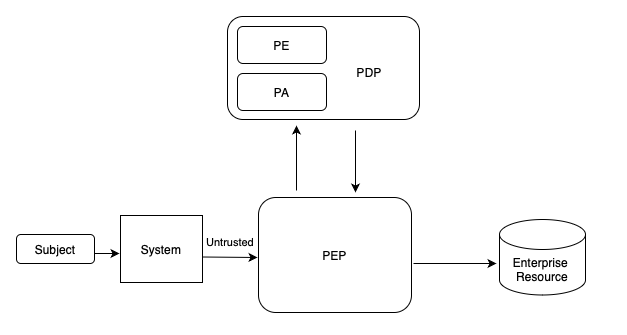
\includegraphics[height=5cm]{./images/architecture}
  \caption{Logical components of ZTA[source: NIST]}
  \label{fig:architecture}
\end{figure}


\subsubsection{Policy Engine}
The PE is in charge of deciding whether or not to allow access to a resource for a particular resource.
To give, deny, or revoke access to a resource, the PE employs enterprise policy together with input from external sources 
as input to a trust algorithm. The component of the policy administrator is matched with the PE. 
The decision is made by the policy engine, which also documents its approval or rejection. 
The policy administrator then puts the decision into action.

\subsubsection{Policy Administrator}
The PA is the component handling initiation and/or termination of the communication line between a resource and a subject. 
Any session-specific authentication, credential, or token 
that a client uses to get access to an enterprise resource would be generated by it. It is directly related to the PE and 
depends on its final determination of whether to approve or reject a session. The PA sets up the PEP to permit the session 
to begin if the request has been authenticated and the session is allowed. The PA notifies the PEP to terminate the connection 
in the event that the session is rejected or an earlier approval is overturned.

\subsubsection {Policy Enforcement Point}
The PEP is in charge of permitting and overseeing connections between a subject and an enterprise 
resource. The PEP interacts with the PA in order to transmit requests and/or 
obtain updates on PA policies. Although there is just one logical component in ZTA, it can be divided into two parts: the 
resource side (such as the gateway component in front of the resource that regulates access) and the client 
(such as an agent on a laptop) or a single portal component that serves as a gatekeeper for communication channels. 
The trust zone containing the enterprise resource is located beyond the PEP, as seen in figure 2.1.

[cite NIST here]

\section{Kubernetes}

\subsection{Components}

A Kubernetes cluster is separated into a control plane and data plane. The control plane
groups the components responsible for the underlying system of Kubernetes itself. The data
plane hosts the actual user containers. Machines that run control-plane services are referred to as master-nodes, 
whereas machines that host user applications are referred to as worker-nodes. There are four core control-plane components
 which work together to manage the cluster and ensure that applications run smoothly. These components run as containers
themselves inside the reserved ’kube-system’ namespace. 
\newline
\begin{figure}[htbp]
  \centering
      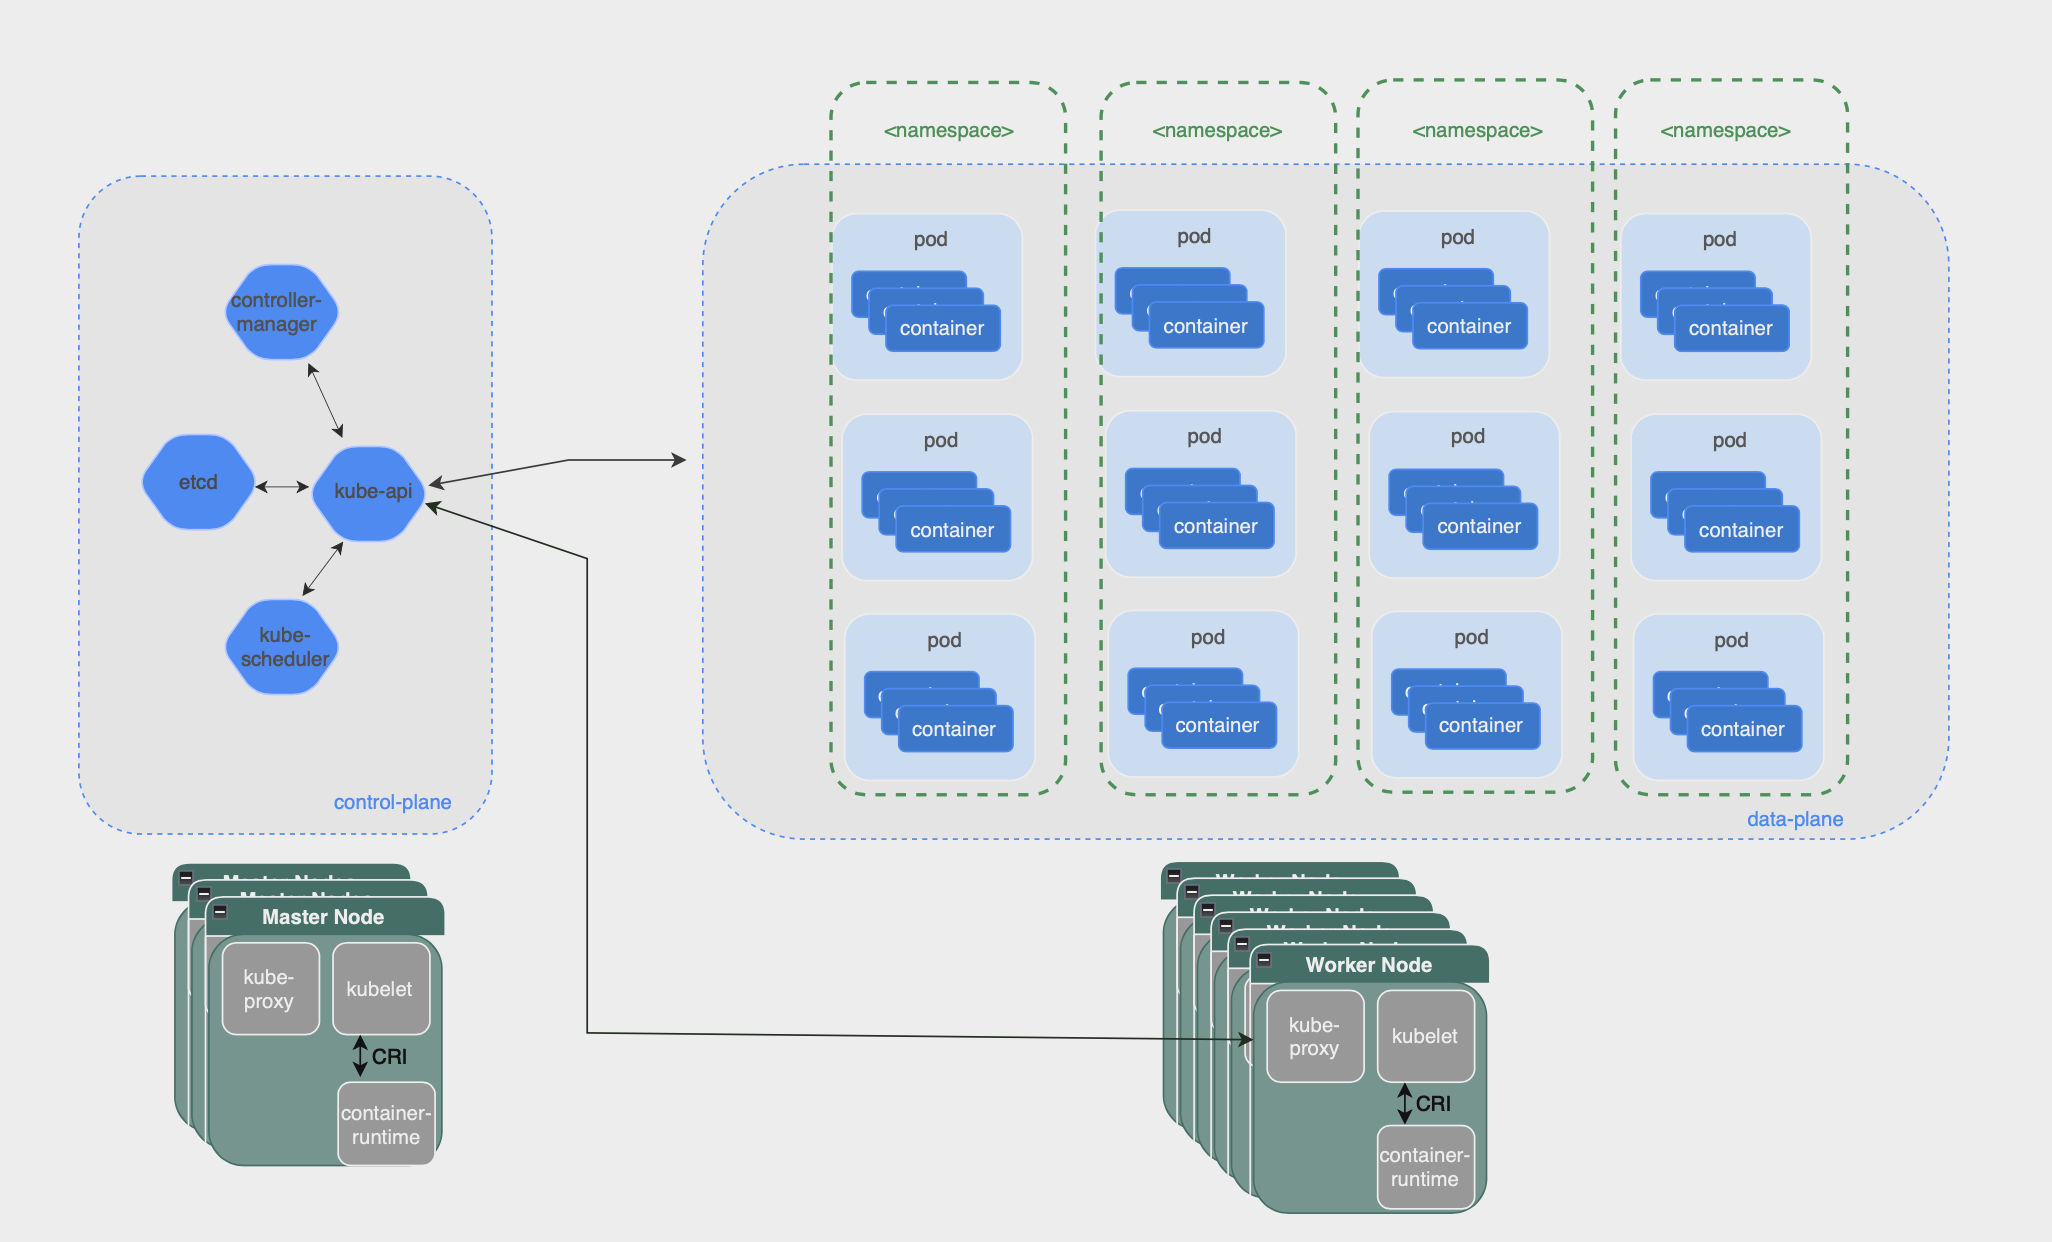
\includegraphics[height=8cm]{./images/kubernetes}
  \caption{Kubernetes Architecture [source: author]}
  \label{fig:architecture}
\end{figure}
\newline
The API server in Kubernetes acts as the gateway, offering a REST API 
through which users and applications can communicate with the cluster, enabling resource management, access control, and 
querying of cluster state and configurations. The Kubelet, an agent process on each node, ensures that pods are running healthy
and up-to-date with the desired state. It does so by communicating with the API server.
Etcd, a distributed key-value store, maintains the cluster's consistent state across multiple nodes, utilized by control plane
components for storing cluster information like resource configurations and pod statuses.
The kube-scheduler allocates pods to nodes based on resource availability and requirements, aiming to optimize successful pod 
execution while enhancing cluster resilience by distributing pods across multiple nodes.
The controller manager, operating on each node, oversees the cluster's state, responds to events like pod creation or deletion, and does 
corrective measures to maintain cluster health, such as restarting unhealthy pods or scaling to meet demand. [cite k8s docs]

\subsection{Core Cluster Objects}

\subsubsection{Namespaces}
Within a single cluster, resource groups are arranged and separated using namespaces, which are virtual partitions in Kubernetes. 
Namespaces allow the cluster to be logically divided into smaller, more manageable chunks. 
Namespaces are used by Kubernetes objects like "Deployment," "Service," and "ConfigMap" to describe an application's state. 
Globally existing and not namespaced objects are those that define the cluster as a whole or that apply to all applications across all namespaces. 
Namespace isolation preserves the integrity of every deployment by averting unintentional interactions or interference between applications. 
Custom authorization rules and access control techniques can be enforced by assigning distinct security policies to namespaces. 
This aids in resource protection and limits unauthorised access between specific namespaces inside the cluster. [cite k8s docs]


\subsubsection{Pods, Replicasets, Deployments, Statefulsets}

In Kubernetes, pods are fundamental building blocks for deploying and managing container-
ized applications. A pod is a unit of one or more containers, which belong together and share
resources such as network namespaces and filesystems. This tight coupling allows pods to be
treated as a single unit for scheduling, management, and resource allocation. Pods expose
the ports exposed by its containers, allowing external traffic to reach its intendend recipient.
Pods are rarely instantiated by itself. Deployments, Replicasets and Statefulsets are higher 
deployment configurations which specify pod settings. [cite k8s docs]

\subsubsection{ServiceAccount and RBAC}

Pods can use a ServiceAccount as a security identity to access Kubernetes services and resources. 
It controls pod access permissions and interactions with the cluster and serves as an authentication method for pods. 
ServiceAccounts have the ability to mount Secrets into Pods, giving them access to private information like certificates, API keys, and passwords.
\newline
RBAC is an authorization system that regulates which individuals or groups are able to access resources and carry out particular tasks inside the cluster. 
It offers a detailed method for controlling access rights and enforcing security regulations throughout the Kubernetes environment.
Role objects define a set of permissions that can be granted to users or groups. They specify which resources can be accessed, what actions can be performed 
on those resources, and the scope of the permissions (namespace-wide or cluster-wide). ClusterRole objects are similar to Roles, but they have a broader scope, 
applying to all namespaces within the cluster. They are typically used to define permissions for system components or users who need access to resources across multiple namespaces.
RoleBindings and ClusterRoleBindings assign the designated permissions to users or groups based on the association between Roles or ClusterRoles. 
They specify how identities and the permissions they possess are mapped out. Such RoleBindings are bound to previously mentioned ServiceAccounts. [cite k8s docs]


\subsection{Kubernetes Networking}

A key component of Kubernetes that guarantees smooth communication between containers, pods, and services inside a Kubernetes cluster is Kubernetes networking. 
Networking is made uniform by the Kubernetes network model.

\subsubsection{Pod Networking}
Each pod in Kubernetes has its own IP address, containers within a pod can freely communicate with one another via localhost. With these pod IP addresses, pods 
can communicate with any other pod in the cluster without requiring Network Address Translation (NAT). Network policies are used to establish pod isolation; 
pods are treated in the same way as virtual machines (VMs) or hosts with distinct IP addresses. Because they operate in the same network namespace, containers inside of 
pods share the IP address of the pod.

\subsubsection{Service and Ingress}
Access to a collection of pods is abstracted by Kubernetes services and is often represented by a virtual IP address within the cluster. Node ports or load balancers 
allow access to these services from outside the cluster. Even when the underlying pods change, a service's virtual IP address and DNS name stay the same. Load balancing and 
flexible access control are thus made possible.

\subsubsection{Container Network Interface (Plugins)}
The Container Network Interface (CNI) API provided by Kubernetes allows for the support of several network solutions. Third-party network implementations are increasingly
utilized, even though Kubernetes' integrated network support, kubenet, provides basic connectivity. Pods can be connected to the network using network plugins, and pod IP addresses 
can be assigned using IP Address Management (IPAM) plugins. Calico and Cilium, for instance, offer flexibility in selecting the optimal networking solutions for certain needs and settings by 
providing both network and IPAM plugins and integrating with other CNI plugins.

[cite tigera, cilium, k8s docs]



\chapter{Creating the cluster}

\section{Virtual Machines and Network}

The base infrastrucure of the thesis project consists of 5 Virtual Machines which are running on a Proxmox infrastructure provided by FH Campus Wien. At the edge of the network sits an OPNsense 
gateway, an open-source firewall based on FreeBSD, which controls external traffic coming into 
this thesis' network. Its external interface on 10.140.0.50 is part of a broader WAN provided by institution's facilities. This gateway serves as the primary entry and exit point for all traffic 
entering or leaving the internal network, playing a critical role in securing and directing network traffic. The gateway runs a Wireguard agent - the general environment is accessed using SSH through  
a Wireguard VPN tunnel. As this thesis focuses on the Kubernetes environment, and as OPNsense is not directly 
part of the Kubernetes setup, there shall be no further in-depth description of this OPNsense gateway. 
\newline
\newline
The LAN is segmented into a distinct subnet 192.168.20.0/24. Within this subnet, four VMs have been deployed, each assigned static IP addresses ranging from 192.168.20.1 to 192.168.20.5. 
These VMs serve various roles within the network, hosting different services and agents required for the Kubernetes environment and its Zero Trust character. A static IP address assignment was chosen to ensure consistent network addressing, 
and to facilitate easier management and configuration of these VMs. The Ubuntu installation wizard was used to complete base configurations such as username, password, hostname and IP addresses. 
Each of these VMs runs Ubuntu 22.04 LTS, a popular Linux distribution known for its stability, security features, and extensive software repositories. 
This choice of operating system emphasizes a preference for a robust, community-supported platform capable of handling the demands of modern networked applications. 
With 8GB of RAM and 4 CPU cores allocated to each VM, they are well-equipped to run Kubernetes.
\newline
\newline
To give a general introduction of the setup, an authentication proxy is deployed on a standalone VM on 192.168.20.2, apart from the Kubernetes cluster itself. The cluster is deployed on the remaining three 
VMs. 192.168.20.3, the master node, is running the control-plane (the "brain" of the cluster), consisting of kube-apiserver, etcd, kube-controller-manager and kube-scheduler. 192.168.20.4 and 192.168.20.5 are dedicated worker 
nodes of the cluster running the data-plane (the "body" of the cluster), hosting deployed containers. Each node runs the Kubelet and the kube-proxy. The cluster is organized in multiple namespaces. The components
and software solutions which ensure a Zero Trust approach are deployed in their respective, dedicated namespaces, such as istio-system, keycloak and teleport-agent, for example. To mimick actual business software hosted on Kubernetes
and for the sake of demonstration, namespace "neptune" and namespace "jupiter" are created. Each of them run simple deployments such as a Nginx webserver. This setup, as shown in figure 3.1, will be explained in depth in the following sections. 

\begin{figure}[htbp]
  \centering
      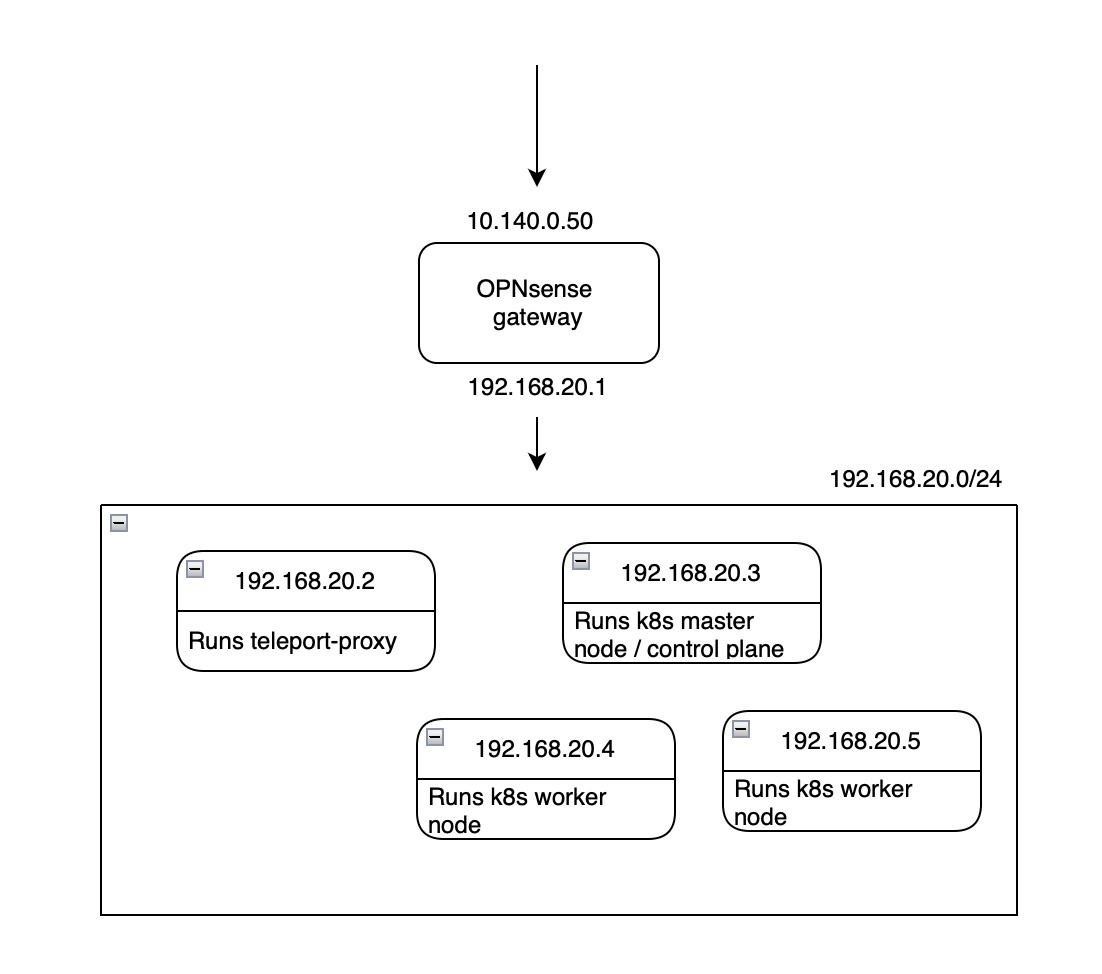
\includegraphics[height=8cm]{./images/setup}
  \caption{General Setup [source: author]}
  \label{fig:generalsetup}
\end{figure}



\section{Bootstrapping the cluster with kubeadm}

Before installing Kubernetes binaries on the nodes, certain settings and kernel parameters need to be configured on the Linux machines that make up the Kubernetes nodes. 
The bash script as seen in figure 3.2 is executed on all three nodes.
\newline
\begin{figure}[htbp]
  \centering
      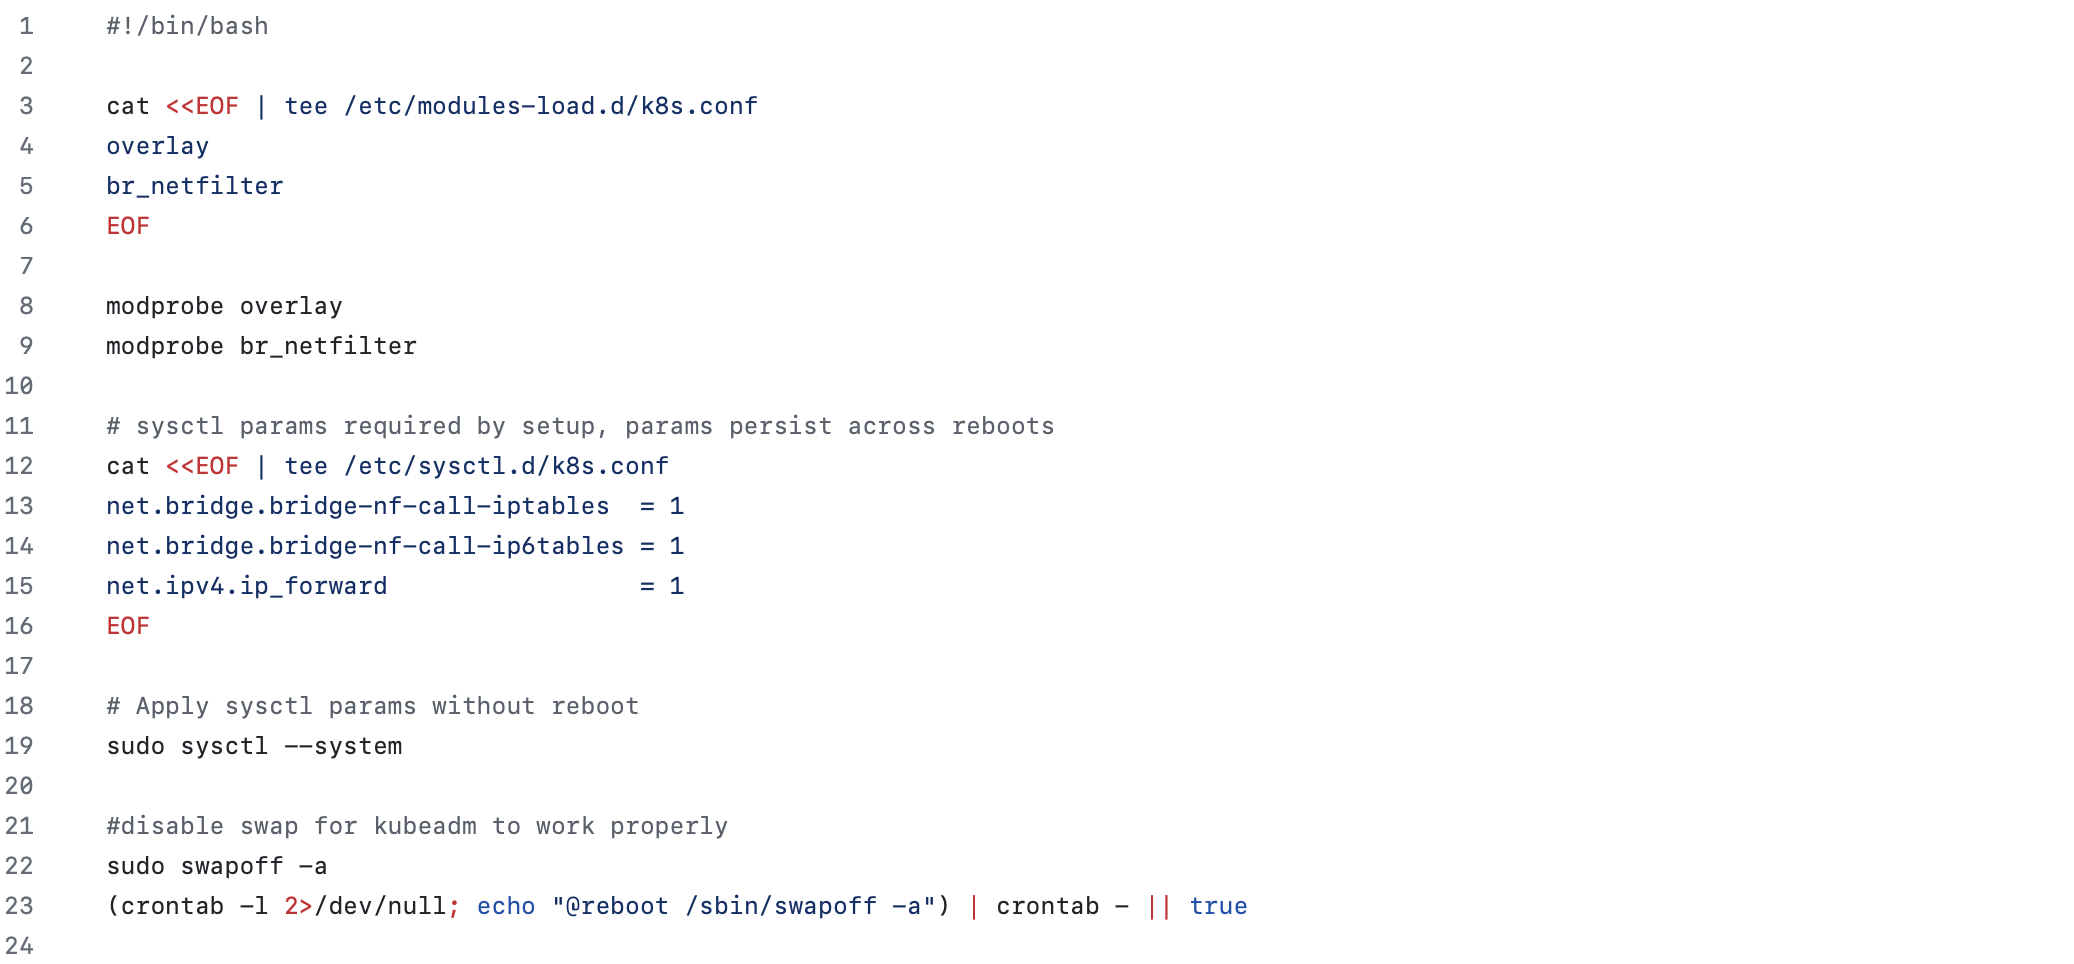
\includegraphics[height=7.8cm]{./images/baseconfig}
  \caption{Base k8s-node configuration [source: author]}
  \label{fig:baseconfig}
\end{figure}
\newline
This script places a k8s.conf file under the /etc/modules-load.d/ directory, specifying overlay and bridge netfilter. This ensures that the kernel modules overlay and bridge netfilter are always loaded at startup of the VM, 
which are required for Kubernetes networking and storage requirement.

\subsubsection{Overlay}
The overlay module is essential for Kubernetes because it activates the overlay storage driver used by container runtimes such as Docker to manage container filesystems efficiently. 
This driver allows containers to share and layer filesystems, optimizing storage use and enhancing performance. By enabling the overlay module, Kubernetes ensures that container runtimes 
can efficiently create, manage, and run containers, which is crucial for the effective functioning of the cluster.

\subsubsection{Bridge Netfilter}
The bridge netfilter module is important because it allows the Linux bridge to interface with the iptables firewall, enabling packet filtering and NAT. 
This capability is needed for Kubernetes to manage and route network traffic between pods, services, and external networks efficiently. net.bridge.bridge-nf-call-iptables and net.bridge.bridge-nf-call-ip6tables
settings ensure that bridged traffic goes through the iptables chains. net.ipv4.ip-forward enables IP forwarding, allowing the Linux kernel to forward packets between (virtual) network interfaces.
\newline
\newline
With the modprobe command, these modules are loaded into the kernel and their functions are made available.
Without these settings, Kubernetes components may experience problems with container filesystem management, network packet processing, and general traffic routing.

\subsubsection{Swap}
Disabling swap on Linux during Kubernetes setup, as done in lines 22-23 of figure 3.2, is necessary because Kubernetes depends on efficient memory management for container orchestration. 
When swap is active, the kernel might swap container memory to disk. 
This results in unpredictable performance and potential container instability. By turning off swap, Kubernetes ensures that container memory stays in physical RAM. 
This allows Kubernetes to manage containers effectively without interference from swapping mechanisms.



\newpage
\section{Protocols and standards}

\subsection{OpenID Connect}

OpenID Connect serves as a straightforward identity service that builds upon the OAuth 2.0 framework. It enables client applications to authenticate users through an authorization server or identity provider (IdP) and retrieve essential 
client profile details in a standardized, RESTful approach. This service defines a RESTful HTTP API that utilizes JSON for data exchange.

Explain Oauth2 and OpenID connect and then say the same can be done for app to app communication


\subsection{Multi-Factor Authentication}
\subsection{mTLS}


\section{Teleport: Access to the cluster with commandline clients}

\section{Istio: Handling app-communication using a service-mesh}

\section{Keycloak: Implementing OIDC}

\section{Keycloak and Istio: AuthorizationPolicy and RequestAuthentication, python OIDC client with tokens}

\section{Vault: Centralized secret management}

\section{Monitoring}

\section{Trivy: Continuous scanning}

\section{}

\newpage
\chapter{Discussion and Future Work}

\chapter{Conclusion}

\newpage

% --- Bibliography ------------------------------------------------------

%IEEE Citation [1]
\bibliographystyle{IEEEtran}
%for alphanumeric citation eg.: [ABC19]
%\bibliographystyle{alpha}

% List references I definitely want in the bibliography,
% regardless of whether or not I cite them in the thesis.

\newpage
\addcontentsline{toc}{chapter}{Bibliography}
\bibliography{testBib}

\newpage

% --- List of Figures ----------------------------------------------------

\addcontentsline{toc}{chapter}{List of Figures}
\listoffigures


% --- List of Tables -----------------------------------------------------

\newpage
\addcontentsline{toc}{chapter}{List of Tables}
\listoftables

% --- Appendix A -----------------------------------------------------

\backmatter
\appendix
\begin{appendices}
\chapter{Appendix}

(Hier können Schaltpläne, Programme usw. eingefügt werden.)

\clearpage
\end{appendices}

\end{document}
